% Questo file contiene la domanda e risposta sul Modello ER, Normalizzazione e SQL per Corsi/Docenti/Appelli.
% Sarà incluso da domande_ed_esercizi_bd.tex.

\subsection*{Domanda: Modello ER, Normalizzazione e SQL (Corsi, Docenti, Appelli)}

\textbf{Domanda}: Il candidato descriva il modello concettuale Entità-Relazione (ER) e il concetto di forma normale nella progettazione logica. Produca un diagramma ER che rappresenti il contesto seguente: "Un corso è associato a un docente titolare e può includere più appelli d'esame durante l'anno accademico. Ogni appello d'esame può avere uno o più studenti iscritti." Successivamente il candidato fornisca una progettazione in forma tabellare del modello, normalizzando le relazioni, fornendo infine una query SQL per ottenere l'elenco di tutti gli iscritti a un determinato appello d'esame.

\paragraph{Risposta}:

\textbf{Descrizione del Modello Concettuale Entità-Relazione (ER)}
Il \textbf{Modello Entità-Relazione (ER)} è uno strumento di alto livello per la progettazione concettuale di database. Permette di rappresentare il mondo reale tramite entità (oggetti o concetti di interesse) e relazioni (associazioni tra entità). I suoi componenti principali sono:
\begin{itemize}
    \item \textbf{Entità}: Cose o oggetti reali (es. Studente, Docente). Rappresentate con rettangoli.
    \item \textbf{Attributi}: Proprietà delle entità o relazioni (es. Nome, CodiceFiscale). Rappresentati con ovali. Possono essere semplici, composti, multi-valore, derivati o chiavi (sottolineate).
    \item \textbf{Relazioni}: Associazioni logiche tra entità (es. Insegnare, Iscrizione). Rappresentate con rombi. Hanno cardinalità (min:max) e partecipazione.
\end{itemize}

\paragraph{Concetto di Forma Normale nella Progettazione Logica}
La \textbf{normalizzazione} è un processo di organizzazione dei dati in un database relazionale per ridurre la ridondanza e migliorare l'integrità dei dati. Si basa sulle forme normali:
\begin{itemize}
    \item \textbf{Prima Forma Normale (1NF)}: Tutti gli attributi sono atomici e ogni record è unico.
    \item \textbf{Seconda Forma Normale (2NF)}: È in 1NF e tutti gli attributi non-chiave dipendono completamente dalla chiave primaria (no dipendenze parziali).
    \item \textbf{Terza Forma Normale (3NF)}: È in 2NF e non contiene dipendenze transitive (nessun attributo non-chiave dipende da un altro attributo non-chiave).
\end{itemize}

\paragraph{Diagramma ER per il Contesto Specifico}
Il contesto da modellare è: "Un corso è associato a un docente titolare e può includere più appelli d'esame durante l'anno accademico. Ogni appello d'esame può avere uno o più studenti iscritti."

\begin{figure}[h!]
    \centering
    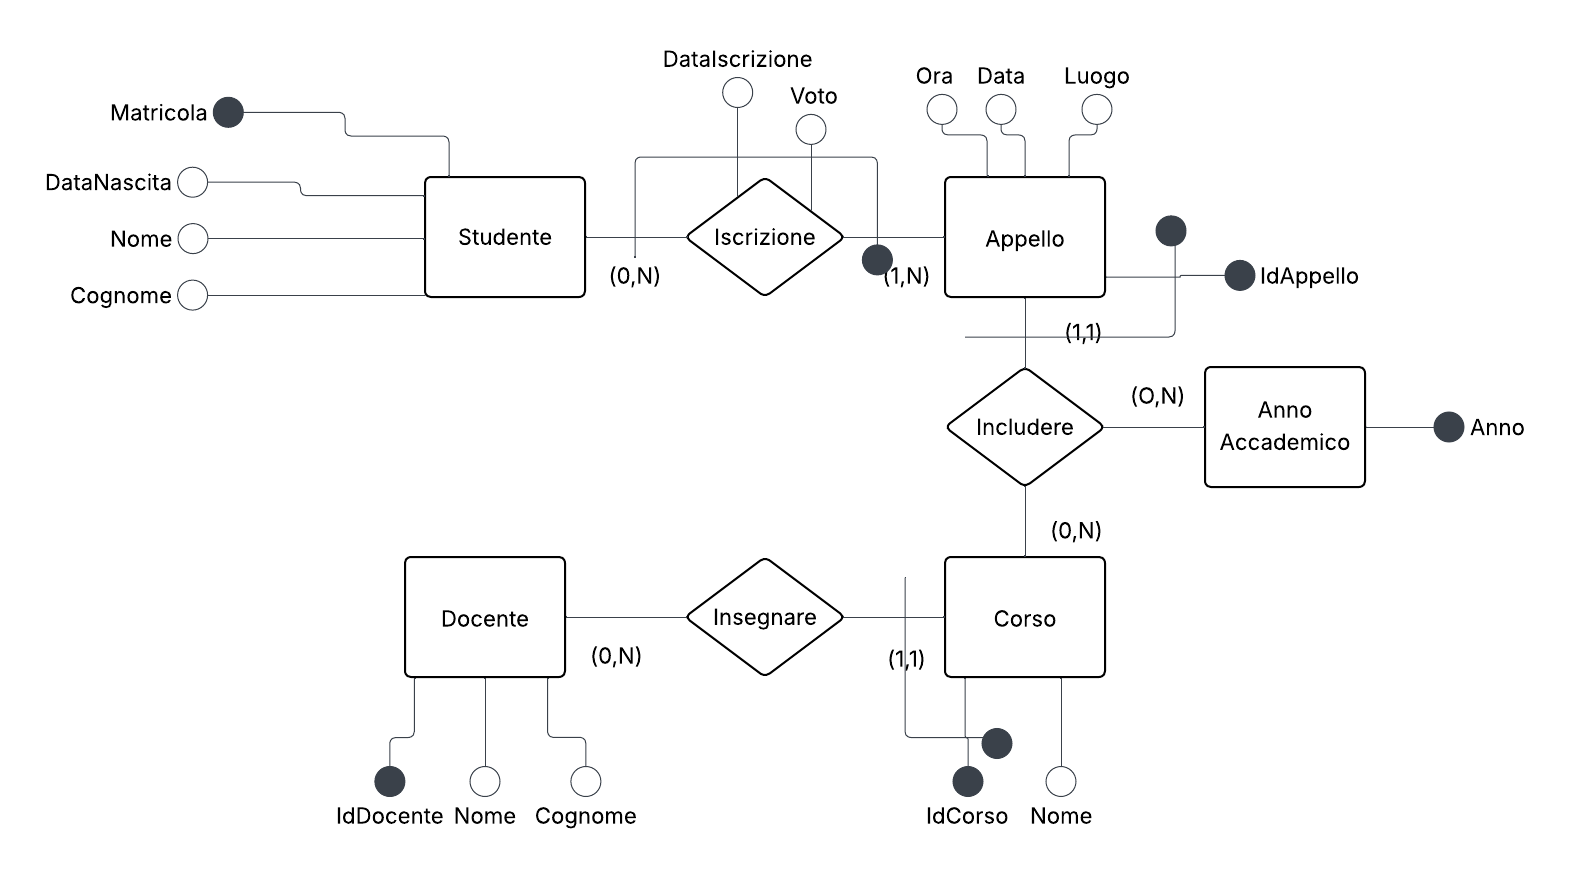
\includegraphics[width=0.9\textwidth]{capitoli/basi_di_dati/domande_teoriche/immagini/er_esame_stato_corsi_docenti_appelli.png}
    \caption{Diagramma Entità-Relazione per la gestione di corsi, docenti, appelli d'esame e studenti.}
    \label{fig:er_esame_stato_corsi_docenti_appelli}
\end{figure}

\textbf{Spiegazione del Diagramma:}
\begin{itemize}
    \item \textbf{Entità}: `Studente`, `Appello`, `Docente`, `Corso`, `Anno Accademico`.
    \item \textbf{Attributi impliciti/necessari}: Per completezza, assumiamo per `Studente` (Matricola PK, Nome, Cognome), per `Appello` (IDAppello PK, Data, Ora, Luogo), per `Docente` (IDDocente PK, Nome, Cognome), per `Corso` (IDCorso PK, NomeCorso) e per `Anno Accademico` (Anno PK).
    \item \textbf{Relazione "Iscrizione" (Studente - Appello)}: È una relazione N:M. Un `Studente` può iscriversi a zero o più `Appelli` (`(0,N)` lato Studente). Un `Appello` deve avere uno o più `Studenti` iscritti (`(1,N)` lato Appello). Potrebbe avere attributi sulla relazione come `Voto`, `DataIscrizione`.
    \item \textbf{Relazione "Insegnare" (Docente - Corso)}: È una relazione 1:N. Un `Docente` può insegnare a zero o più `Corsi` (`(0,N)` lato Docente). Un `Corso` è insegnato da uno e un solo `Docente` (`(1,1)` lato Corso), indicando il docente titolare.
    \item \textbf{Relazione "Includere" (Corso - Appello - Anno Accademico)}: Questa è modellata come una relazione ternaria. Un `Corso` può avere zero o più `Appelli` in un dato `Anno Accademico` (`(0,N)` lato Corso). Un `Appello` è sempre legato a uno e un solo `Corso` e a un solo `Anno Accademico` specifico (`(1,1)` lato Appello). Un `Anno Accademico` può includere zero o molti `Appelli` di `Corsi` (`(0,N)` lato Anno Accademico). Questa modellazione ternaria cattura il vincolo che un appello di un corso si tiene in un determinato anno accademico.
\end{itemize}

\paragraph{Progettazione in Forma Tabellare (Modello Relazionale Normalizzato)}
Traducendo lo schema ER in uno schema relazionale e applicando la normalizzazione (fino alla 3NF):

\begin{itemize}
    \item \textbf{DOCENTI} (\underline{IDDocente}, Nome, Cognome)
    \item \textbf{CORSI} (\underline{IDCorso}, NomeCorso, IDDocenteFK)
    \item \textbf{ANNI\_ACCADEMICI} (\underline{Anno})
    \item \textbf{APPELLI} (\underline{IDAppello}, Data, Ora, Luogo, IDCorsoFK, AnnoAccademicoFK)
    \item \textbf{STUDENTI} (\underline{Matricola}, Nome, Cognome, DataNascita)
    \item \textbf{ISCRIZIONI} (\underline{MatricolaFK, IDAppelloFK}, DataIscrizione, Voto)
\end{itemize}

\textbf{Motivazione della Normalizzazione}:
\begin{itemize}
    \item Tutte le tabelle sono in 1NF (attributi atomici, PK unica).
    \item Poiché non ci sono chiavi primarie composte in \lstinline{DOCENTI}, \lstinline{CORSI}, \lstinline{ANNI_ACCADEMICI}, \lstinline{APPELLI}, \lstinline{STUDENTI}, queste sono automaticamente in 2NF. Non ci sono dipendenze transitive, quindi sono in 3NF.
    \item Per \lstinline{ISCRIZIONI} (chiave composta: \lstinline{MatricolaFK}, \lstinline{IDAppelloFK}), gli attributi \lstinline{DataIscrizione} e \lstinline{Voto} dipendono da \textit{entrambe} le parti della chiave, quindi è in 2NF. Non ci sono dipendenze transitive, quindi è in 3NF.
    \item Questa scomposizione riduce la ridondanza (es. nomi di corsi/docenti non ripetuti in \lstinline{APPELLI}) e previene anomalie di aggiornamento, inserimento e cancellazione.
\end{itemize}

\paragraph{Query SQL per l'Elenco degli Iscritti a un Determinato Appello d'Esame}
Supponiamo di voler ottenere l'elenco di tutti gli studenti iscritti all'appello d'esame con `IDAppello = 'APP2025-001'`.

\begin{lstlisting}[language=SQL, caption={Query per l'elenco degli iscritti a un appello d'esame specifico}]
SELECT
    S.Nome AS StudentFirstName,
    S.Cognome AS StudentLastName,
    S.Matricola AS StudentMatricola,
    A.Data AS ExamDate,
    A.Ora AS ExamTime,
    C.NomeCorso AS CourseName
FROM
    STUDENTI S
JOIN
    ISCRIZIONI I ON S.Matricola = I.MatricolaFK
JOIN
    APPELLI A ON I.IDAppelloFK = A.IDAppello
JOIN
    CORSI C ON A.IDCorsoFK = C.IDCorso
WHERE
    A.IDAppello = 'APP2025-001';
\end{lstlisting}
Questa query connette le tabelle `STUDENTI`, `ISCRIZIONI`, `APPELLI` e `CORSI` per recuperare i dettagli degli studenti e dell'appello/corso corrispondente, filtrando per un ID di appello specifico.